\documentclass{article}
\usepackage[utf8]{inputenc}
\usepackage{titling}

\setlength{\droptitle}{-5em}   % This is your set screw
\usepackage[margin=3.0cm]{geometry}
\usepackage{caption}
\usepackage{graphicx}
\usepackage{subcaption}
\usepackage{fixltx2e}
 
\title{Evaluating the Performance Characteristics of Opportunistic Routing Protocols during an Emergency Fire \& Rescue Scenario involving a High-Density Cluster of Victims}
\author{
  Oliver Mitchell\\
  \texttt{psyom1@nottingham.ac.uk}\\\\
  \textnormal{School of Computer Science}\\
  \textnormal{University of Nottingham}
}
\date{December 12th, 2018}
 
\begin{document}

\maketitle
 
\tableofcontents
\newpage

\section{Introduction}
The aim of this project is to evaluate the performance characteristics of 2 different opportunistic routing protocols within a real world scenario, simulated by the Opportunistic Network simulator (ONE). In the chosen scenario, victims of an arson attack are trapped within a museum, trying to contact the local hospital. The scenario is simulated by a network topology that represents the city of Helsinki and its transport network. The simulation was designed to mimic real-life scenarios which involve large amounts of active mobile devices in close proximity to each other in an enclosed space (high-density clusters).\\
\newline
To begin, this paper will give a brief overview of opportunistic networks and the 2 routing protocols evaluated in the experiment. Then, the functionality of the ONE simulator will be described and the model of the scenario explained in detail, including its implementation. Using this model, simulations will be run and the results of their performances critically evaluated. A conclusion will then be drawn based on these results, summarising the pros and cons of both routing protocols and their use in the observed scenario. Finally, the paper closes with a wider discussion of the usefulness of opportunistic networks in related real world use-cases.

\section{Background}
In recent years, a growing number of devices have been utilizing mobile networking technology in less traditional environments, ranging from the GPS tracking of wildlife over huge distances [4], to the proposed establishment of an "Interplanetary Internet", capable of transmitting data lightyears in distance [5]. These non-static networks are decentralised and wireless, consisting of constantly mobile nodes, ranging from those with predictable mobility, such as transport systems, (e.g. buses and trams) to those with stochastic mobility, such as military/tactical networks. In all of these new environments, communication coverage is pervasive and essential for day-to-day operations. However, it's impossible to treat them like traditional networks with pre-determined communication paths due to their constant reconfiguration and non-guaranteed connectivity. As a result, computer networks deployed in such environments face new challenges such as large delays, intermittent communication links, and heterogeneous nodes with differing operating systems and network protocols.

\subsection{Mobile Ad-Hoc Networks (MANETs)}
A Mobile Ad-Hoc Network (MANET) is a self-configuring network of mobile devices, with no fixed infrastructure, connected by wireless links. An important characteristic of a MANET is each node's ability to move independently in any direction, forcing the network to reconfigure itself frequently. Each node acts as a client, server, and router simultaneously in order to transport packets from source to destination, thus nodes communicate with each other in a peer-to-peer fashion [7]. There are several important properties that limit the effectiveness of MANETs [6]:
\begin{itemize}
	\item Security is difficult to achieve because wireless links are vulnerable, the topology is dynamically changing, and there is no certification authority [8].
	\item The use of wireless links results in a lower capacity than wired counterparts [6].
	\item Nodes are mobile devices which rely on exhaustible battery power. Therefore, saving energy is an important system design aspect [6].
\end{itemize}
MANETs assume high connectivity and established routes for transmitting data between nodes in a multi-hop fashion. As a result, the routing process in MANETs requires the discovery of an end-to-end path before data can be transported. However, because the topology is constantly changing in most mobile ad-hoc networks, there may not always be a feasible end-to-end path between source and destination [6]. Resultantly, MANETs perform poorly when connections are intermittent or there are long delays. This problem presents the need for the improved protocols used in opportunistic networks such as Delay Tolerant Networks (DTNs).

\subsection{Vehicular Ad-Hoc Networks (VANETs)}
Vehicular Ad-Hoc Networks (VANETs) are a type of MANET where the network's nodes are represented by vehicles. Though MANETs and VANETs share many characteristics, there are unique challenges exclusive to VANETs that affect their usability, efficiency, and therefore their system design [9]:
\begin{itemize}
	\item Vehicles have the potential to move at very high speeds which can reduce the length of time available for packet transfer between nodes communicating in close proximity to each other [9]. As VANETs also require end-to-end paths to be established before data can be sent, this issue is compounded by the movement of intermediary nodes in multi-hop transmissions. An end-to-end path may be established before transmission begins, but disrupted before the packet can reach its destination.
	\item The data transmitted by vehicles may be critical and life-saving, such as information about road accidents and traffic or the location of casualties who need assistance from ambulance crews. It is therefore essential that such information is received correctly and in a timely fashion [9].
\end{itemize}
It is useful to note that the movement of nodes in a VANET can be considered more predictable than coventional ad-hoc networks because vehicles follow set paths such as roads, railway lines, etc.

\subsection{Delay/Disruption Tolerant Networks (DTNs)}
In environments where disruptions and delays are expected, traditional networking protocols such as TCP [3] are unsuitable because they assume there is an end-to-end connection with low message loss and minimal delay [2]. In decentralised, mobile ad-hoc networks, nodes are constantly moving and there is likely no feasible end-to-end path between source and destination. In order to combat the challenges presented by delays and disruptions, the assumption of an existing end-to-end path from source to destination is dropped. Instead, routing protocols have been developed which utilise a ``store-and-forward'' approach [2][19] where data is gradually transported in single hops and stored in different nodes with the desire of eventually reaching its intended destination. Typically, this approach to network architecture is called Delay/Disruption Tolerant Networking (DTN).\\
\noindent The performance of a DTN depends on the routing protocol used in a given scenario. DTN routing protocols can either be replication based (flooding) or forwarding based [10]:\\
\begin{itemize}
	\item In a replication based protocol, when one node encounters another it will forward a copy of its message without deleting its own. This means there are multiple copies of the message in the network with aims to increase the probability that a message will eventually reach its destination. However, in this approach a large number of resources are used, particularly buffer space. Once the message has been delivered, all existing copies of the message are made redundant but still continue to exist, taking up unecessary space [10].
	\item In a forwarding based protocol, a message can only be stored by a single node at a time. In constrast to a replication based scheme, the node forwarding the message deletes its own copy, making the receiver the sole custodian of the message. Forwarding based protocols tend to use heuristics to evaluate encountered nodes and work out which path is most likely to get the message to its destination the quickest.
\end{itemize}

\subsection{Opportunistic Networks}
With MANETs, VANETs and DTNs explained, it is now possible to define an \textbf{opportunistic network}. Firstly, MANETs (and by extension, VANETs) are NOT considered opportunistic networks [18]. The difference is subtle: MANETs are situated on the network layer of the OSI Model, allowing them full control of routing, leading to assumptions of high-connectivity and the potential creation of established end-to-end routes via intermediaries. They assume that nodes trust each other and are typically deployed in emergency situations. However, opportunistic networks are formed by nodes that do not know or trust each other. They are situated on the application layer of the OSI model which means they have no routing control and may only transport data in a single-hop fashion between neighbouring nodes. DTNs, on the other hand, can be considered opportunistic networks and are typically regarded as their most extreme case. All DTNs (and therefore all opportunistic networks) employ the store-and-forward [2][19] strategy which can be described in the following way:

\begin{figure}[h!]
\captionsetup{justification=centering, font=footnotesize}
\centering
  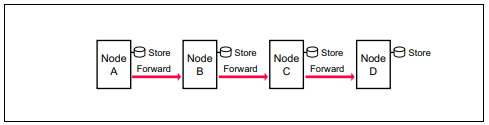
\includegraphics[width=.75\linewidth]{Screenshots/StoreAndForward.png}
  \captionof{figure}{Diagram demonstrating the store-and-forward message passing strategy used in DTNs [19]}
  \label{fig:test1}
\end{figure}

\noindent The store-and-forward strategy is very simple and reminiscent of electronic mail systems. When a node receives a new message, it stores it in its buffer. When that node encounters a relay, it then accesses its buffer and forwards the stored message. This continues in the hope that an encountered node will eventually meet the destination node and deliver the message. The store-and-forward strategy is highly appropriate for networks with unpredictable communication patterns because nodes don't need to know when the next node will come into contact or where it currently is, only to store the data persistently and pass it on when necessary.

\subsection{Delay/Disruption Tolerant Network (DTN) Protocols}
\subsubsection{Epidemic}
Epidemic [11][12] is a simple replication based routing protocol and is somewhat naïve when compared to more advanced protocols. The objective of the epidemic routing protocol is to pass copies of a message to as many nodes as possible in the hope that it eventually reaches its intended destination with minimal delay. Any node that doesn't already have the message will be given a copy and there can exist as many copies of the message as there are nodes in the network. The protocol is called `epidemic' because this indiscriminate method of dissemination is similar to the way in which an infectious disease can propogate through a community; spreading when people come into contact with each other.\\
\newline Theoretically, Epidemic can be seen as an optimal routing protocol if the network's resources are unconstrained. However, in a deployed DTN, the size of each node's message buffer is finite and (because no acknowledgement of receipt is transmitted by the destination node) it is likely that redundant data will still take up unnecessary space in the network. Some research has produced extended versions of the epidemic protocol which mitigate this issue, typically by sending an additional message that confirms receipt and orders 'infected' nodes to delete redundant messages [12].

\begin{figure}[h!]
\captionsetup{justification=centering, font=footnotesize}
\centering
  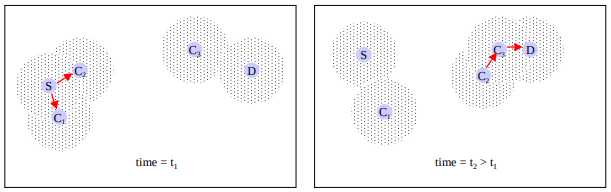
\includegraphics[width=.98\linewidth]{Screenshots/Epidemic.png}
  \captionof{figure}{Diagram showing epidemic message propagation. S is the source node and sends newly encountered nodes C\textsubscript{1} and C\textsubscript{2} message copies at time T\textsubscript{1}. At time T\textsubscript{2}, C\textsubscript{2} encounters a new node, C\textsubscript{3}, and sends it a copy of the message who in turn delivers it to D, the destination. [11]}
  \label{fig:test1}
\end{figure}

\subsubsection{Spray-and-Wait}
Spray-and-Wait [13] is a routing protocol that aims to achieve the advantages of Epidemic's high delivery probability but with far less resource utilisation. It achieves this by disseminating a finite quantity of message copies (spraying) with the recipients storing the message until direct contact with the destination node. The maximum number of messages to spray is typically configured by a variable, \textbf{\textit{L}}. There are 2 versions of the spray-and-wait protocol: vanilla and binary. The difference between them is the method used to disseminate the message copies to \textbf{\textit{L}} different nodes.
\begin{itemize}
	\item \textbf{Vanilla} - transmit one copy of the message to the first \textbf{\textit{L} - 1} nodes encountered. Each node with 1 copy of the message waits until the destination node comes into direct contact.
	\item \textbf{Binary} - start with \textbf{\textit{L}} copies and transmit \textbf{\textit{L}/2} copies to the first node encountered. Both these nodes then transmit \textbf{\textit{n}/2} copies of the message to any new nodes they encounter that do not have the message, where \textbf{\textit{n}} is the total number of messages a node currently holds. When a node has 1 copy remaining, it waits until the destination node comes into direct contact.
\end{itemize}

%\begin{figure}[h!]
%\captionsetup{justification=centering, font=footnotesize}
%\centering
%\begin{minipage}[t]{.5\textwidth}
%  \centering
%  \includegraphics[width=.98\linewidth]{Screenshots/SWBinary.png}
%  \captionof{figure}{Example of binary spray-and-wait message %propagation}
%  \label{fig:test1}
%\end{minipage}%
%\begin{minipage}[t]{.5\textwidth}
%  \centering
%  \includegraphics[width=.98\linewidth]{Screenshots/SWVanilla.png}
%  \captionof{figure}{Example of vanilla spray-and-wait message %propagation}
%  \label{fig:test2}
%\end{minipage}
%\end{figure}

\noindent Binary has an advantage over vanilla because messages are disseminated away from the source at a faster rate [13].

\section{ONE Simulator}
The ONE (Opportunistic Network Environment) Simulator [14][15] is a DTN simulator developed and maintained by researchers on the SINDTN and CATDTN projects and supported by Nokia Research Center (Finland). Where existing DTN simulators focused solely on routing simulation, ONE combines DTN routing, mobility modelling, and visualisation into one package [14]. It is a complex tool that is extensible and provides useful modules for the reporting and analysis of simulated network environments.\\
\newline ONE is useful for comparing, contrasting and analysing the performance of opportunistic networking protocols in different scenarios, making it the ideal tool for this research paper. Scenarios (or network models) are comprised of network nodes (hosts) which all possess user-specified networking interfaces, energy sources, buffer-sizes, and computing power. Collections of identical nodes can be defined as groups with default properties, though an individual node's settings can be overwritten if necessary, for example, to ensure a node uses a different routing protocol from the rest of its group. Nodes act autonomously, passing messages to other nodes within their communication range according to their designated routing protocol.\\ 
\newline ONE also makes a comprehensive framework for the mobility of nodes available to the user, allowing them to customise the travel speed of individual nodes or groups of nodes and even import real-world movement traces for nodes to follow. This high fidelity node mobility framework allows users to easily differentiate between different node types (e.g. pedestrians will move slower than cars and follow a different route) and permits the creation of highly accurate scenarios that use real-world data or hybrid scenarios which combine real traces with user-defined rules.\\

\begin{figure}[h!]
\captionsetup{justification=centering, font=footnotesize}
\centering
\begin{minipage}[t]{.5\textwidth}
  \centering
  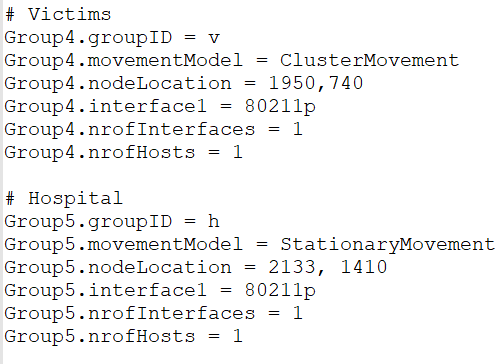
\includegraphics[width=.9\linewidth]{Screenshots/ConfigFileExample.png}
  \captionof{figure}{Screenshot snippet of the ONE simulator's config file}
  \label{fig:test1}
\end{minipage}%
\begin{minipage}[t]{.5\textwidth}
  \centering
  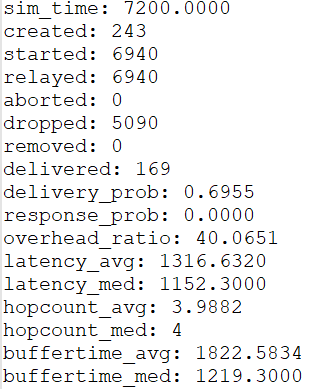
\includegraphics[width=.9\linewidth]{Screenshots/ReportFileExample.png}
  \captionof{figure}{Screenshot snippet of a report file generated by the ONE simulator}
  \label{fig:test2}
\end{minipage}
\end{figure}

\noindent The ONE Simulator allows users to define ``message events'' which are scheduled events involving the creation and movement of messages from source to destination. The user can define the minimum and maximum message size and interval between message creations, a range of source and destination nodes, and a prefix identifier for each message. This system is useful because it allows users to design unique messages for specific scenarios (e.g. one large message sent from a specific node to a specific destination).\\
\newline Creating custom scenarios involves the editing of the ONE simulator's config file. This file contains all the settings that the simulator uses each time it is loaded. It is extremely customisable and allows the user to change the number of nodes, what protocol they use, where they are positioned, how they travel and much more. To simulate a given scenario using ONE, the user needs to ensure the correct config file for that scenario is included as the \texttt{default\_settings.txt} file in the ONE source folder. For this paper, each scenario is represented by an individual config file.\\
\newline The ONE Simulator provides a GUI that allows users to inspect each node present in the model. The user can also inspect the path of individual messages, pause the simulation, and change the speed of the GUI's refresh rate. ONE succeeds in using this GUI to create an accurate visualisation of the user-specified network model. Nodes are clearly represented by prefix identifiers, above an underlayed map image (in this case, an image of Helsinki's transit network). Relationships between nodes are represented by direct lines drawn between them and these constantly update with the simulation's data. Messages in each node's buffer are represented by small stacks of squares next to each node's name. The range of each node's network interface is represented as a green circle. When another node is positioned within this circle, message transfer may commence.\\

\begin{figure}[h!]
\captionsetup{justification=centering, font=footnotesize}
\centering
  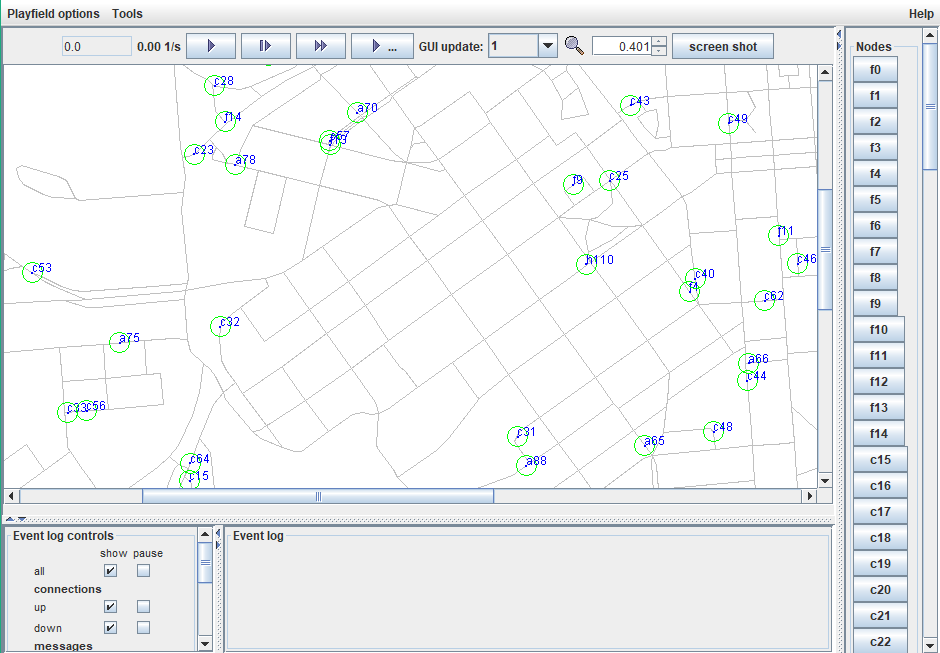
\includegraphics[width=.6\linewidth]{Screenshots/ONEGUI.png}
  \captionof{figure}{Screenshot of the ONE simulator GUI}
  \label{fig:test1}
\end{figure}

\noindent The ONE Simulator provides a comprehensive report feedback system which records many different aspects of a simulation, providing the user with .txt output files. Users can specify which reports to generate in ONE's config file. Examples of reports include statistics on delivery-rate, latency, the number of created connections, and the level of buffer occupancy, just to name a few. The evaluation section of this paper was produced using data from the reports created by each simulation.\\
\newline Finally, the ONE Simulator is open-source and can therefore be extended in any way the user sees fit. This typically includes the modification of existing class files or the creation of new ones. For example, to use an unimplemented routing protocol the user would have to write a new set of source files to include in the software package. The ONE Simulator is very well documented and including new functionality is generally a straightforward process and there are many well-structured classes to inherit from too; the software was built with extension in mind.\\

\section{Experiment}
\subsection{Scenario Description}
The aim of this paper is to evaluate the performance characteristics of the Epidemic and Spray-and-Wait routing protocols within a pseudo-real world scenario. The scenario in question is described in this section:\\
\newline ``Kiasma'', the Helsinki museum of contemporary art, has become the subject of an arson attack conducted by a group of nefarious criminals. Trapped inside the museum are a number of civilian victims who require immediate rescue and assistance from the city's emergency services. In order to do so, the local Helsinki hospital must be contacted. Messages are created by the trapped victims, relayed to vehicles passing local to the museum, and hopefully delivered to their final destination: the Helsinki hospital several streets away.
This scenario has been created using the ONE simulator. However, 3 slightly different versions of the scenario will each be simulated to evaluate how both routing protocols perform. In each scenario the number of trapped victims (and therefore the density of the message source node cluster) is increased. This experiment was designed to to simulate a victim's likely response in such a chaotic scenario: contacting and finding their friends and family who are trapped in the building with them first. Accordingly, messages are likely to be first sent to other victims trapped in the museum before reaching passing vehicles outside.

\begin{center}
\vspace{6px}
\begin{tabular}{|l|p{13cm}|}
\hline
\textbf{Scenario} & \textbf{Description} \\ \hline
\textbf{1} & One trapped victim is simulated by a single node in the network that moves randomly within a small pre-defined range and creates its own messages (Figure 6). \\ \hline
\textbf{2} & 10 trapped victims are simulated by a single node each. Each node moves randomly within a small pre-defined range and is able to create its own messages (Figure 7). \\ \hline
\textbf{3} & 20 trapped victims are simulated by a single node each. Each node moves randomly within a small pre-defined range and is able to create its own messages. \\ \hline
\end{tabular}
\end{center}

\begin{figure}[h!]
\captionsetup{justification=centering, font=footnotesize}
\centering
\begin{minipage}[t]{.5\textwidth}
  \centering
  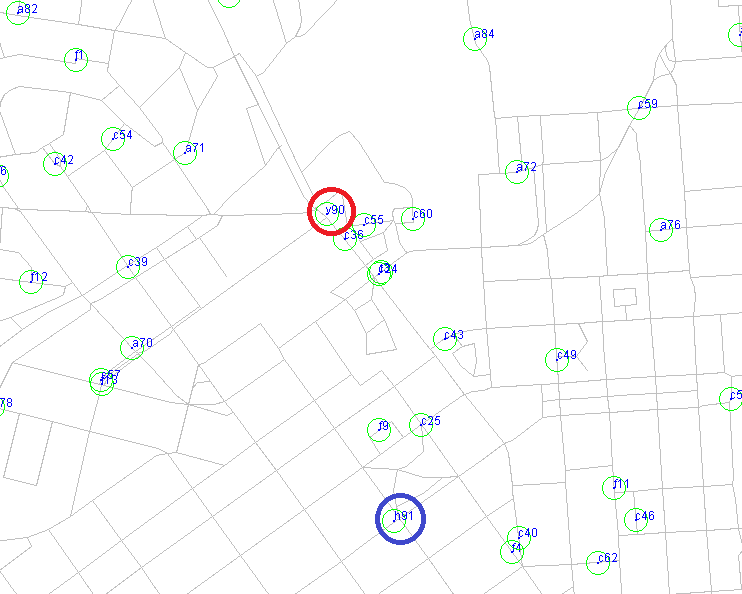
\includegraphics[width=.98\linewidth]{Screenshots/1Node.png}
  \captionof{figure}{Screenshot of the ONE simulator showing a single source node (red circle) and the destination (blue circle)}
  \label{fig:test1}
\end{minipage}%
\begin{minipage}[t]{.5\textwidth}
  \centering
  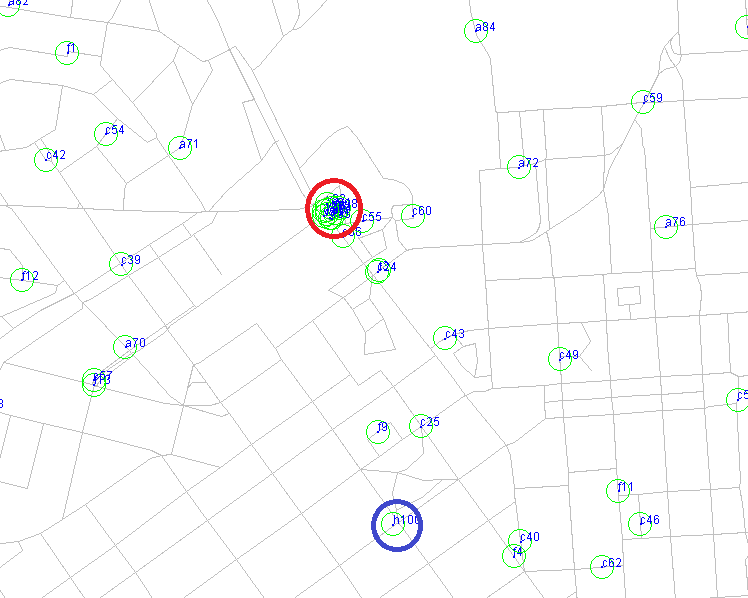
\includegraphics[width=.98\linewidth]{Screenshots/10Nodes.png}
  \captionof{figure}{Screenshot of the ONE simulator showing a high-density cluster of 10 source nodes (red circle) and the destination (blue circle)}
  \label{fig:test2}
\end{minipage}
\end{figure}

\subsection{Assumptions}
The following is a list of assumptions made of the chosen scenario:
\begin{center}
\begin{tabular}{|l|p{13cm}|}
\hline
\textbf{Assumption} & \textbf{Description} \\ \hline
\textbf{1} & All victims (source nodes) are trapped and cannot escape the museum. Their movement is limited to a short range within the building. \\ \hline
\textbf{2} & Each victim has access to their own device which they will use to create emergency messages on the network. \\ \hline
\textbf{3} & Messages created by each victim can be sent to the others victims trapped inside with them. \\ \hline
\end{tabular}
\end{center}

\subsection{Common Simulation Parameters}
Some common settings have been selected for every scenario. All nodes utilise network interfaces which conform to the 802.11p standard [16]. This standard defines wireless access in vehicular environments (WAVE) and is used in the real world for vehicle-to-vehicle communication [16]. A range of 250 metres and a transfer rate of 10MB/s has been selected as a close representation of this standard, taking into consideration limitations such as obstructed signal strength in built-up urban areas. All messages in the simulation represent emergency information which is typically small in size (50-500KB) and uses a relatively short time-to-live (TTL) of 60 minutes. This short TLL ensures large amount of messages do not amass, congesting the network unnecessarily.\\
\begin{center}
\begin{tabular}{|l|l|}
\hline
\textbf{Parameter} & \textbf{Value} \\ \hline
Simulation Time & 120 Minutes \\ \hline
Node Types & People (trapped victims), Cars, Static (Hospital) \\ \hline
Message Size & 50-500KB \\ \hline
Message TTL & 60 minutes \\ \hline
Network Interface & Wi-Fi 802.11p \\ \hline
Network Range & 250 metres \\ \hline
Network Rate & 10MB/s \\ \hline
Buffer Size & 10MB \\ \hline
\end{tabular}
\end{center}

\subsection{Cluster Movement}
To model the trapped victims' movement, the \texttt{movement/ClusterMovement} class was edited. Inside the class, the starting position of node groups using clustered movement was set to the location of the Helsinki museum of contemporary art. Additionally, the range variable was reduced. The node group for the victims uses this edited \texttt{ClusterMovement} class to mimic random movement within a confined space.

\section{Evaluation}
\subsection{Evaluation Criteria Definitions}
The following is a list of the criteria that each routing protocol has been evaluated against:

\begin{center}
\begin{tabular}{|l|p{13cm}|}
\hline
\textbf{Criterion} & \textbf{Description} \\ \hline
Messages Created & The number of unique messages created that must reach their destination (the hospital) \\ \hline
Messages Started & The total number of times the transfer of any message between 2 nodes has started (but not necessarily finished) \\ \hline
Messages Relayed & The total number of times any message has successfully been transferred between 2 nodes \\ \hline
Dropped Messages & The number of messages not relayed by a node due to buffer restrictions \\ \hline
Delivery Probability & Percentage of created messages that have reached their destination \\ \hline
Overhead Ratio & A ratio comparing the number of messages relayed to the number of messages actually delivered, calculated as \texttt{(number of relayed messages - number of delivered messages) / number of delivered messages} \\ \hline
Average Latency & Average time between a message's creation and it reaching its destination \\ \hline
Median Hop Count & The median average number of hops taken for a message to travel from source to destination \\ \hline
\end{tabular}
\end{center}

\subsection{Process of Evaluation}
In each of the 3 scenarios, 3 routing protocols (epidemic, vanilla spray-and-wait and binary spray-and-wait) were tested. Epidemic was tested once for each scenario. Both spray-and-wait versions were tested 5 times each per scenario. For each test, the number of message copies to disseminate was changed with the goal of finding the optimal number of copies. For scenario 2 (cluster of 10 source nodes) the number of copies ranged from 6-30. For scenario 3 (cluster of 20 source nodes) the number of copies ranged from 12-60. These quantities ensured that the difference between the number of message copies and the number of source nodes was proportional across both scenarios.

\newpage

\subsection{Scenario 1}
In this scenario, one trapped victim is simulated by a single node in the network that moves randomly within a small pre-defined range and creates its own messages.

\begin{center}
\captionof{table}{Performance data for the epidemic routing protocol in scenario 1}
\vspace{6px}
\begin{tabular}{|r|c|}
\hline
\textbf{Parameter} & \textbf{Epidemic} \\ \hline
Messages Created & 243 \\ \hline
Messages Started & 56976 \\ \hline
Messages Relayed & 56975 \\ \hline
Messages Dropped & 53841 \\ \hline
Messages Delivered & 99 \\ \hline
Delivery Probability & 40.7\%\\ \hline
Overhead Ratio & 574.5 \\ \hline
Average Latency & 786.4 \\ \hline
Median Hop Count & 6 \\ \hline
\end{tabular}
\end{center}

\begin{center}
\captionof{table}{Performance data for the binary spray-and-wait routing protocol in scenario 1 using different values for the message copy limit}
\vspace{6px}
\begin{tabular}{|r|c|c|c|c|c|}
\hline
\textbf{Parameter} & \textbf{SWB6} & \textbf{SWB12} & \textbf{SWB18} & \textbf{SWB24} & \textbf{SWB30} \\ \hline
Messages Created & 243 & 243 & 243 & 243 & 243 \\ \hline
Messages Started & 1257 & 2667 & 3995 & 5308 & 6580 \\ \hline
Messages Relayed & 1256 & 2666 & 3993 & 5306 & 6578 \\ \hline
Messages Dropped & 821 & 1632 & 2492 & 3459 & 4438 \\ \hline
Messages Delivered & 84 & 122 & 145 & 161 & 166 \\ \hline
Delivery Probability & 34.6\% & 50.2\% & 59.7\% & 66.3\% & 68.3\% \\ \hline
Overhead Ratio & 13.9 & 20.8 & 26.5 & 31.9 & 38.6 \\ \hline
Average Latency & 1302.3 & 1079.5 & 1189.9 & 1076.6 & 1102.1 \\ \hline
Median Hop Count & 3 & 4 & 4 & 4 & 4\\ \hline
\end{tabular}
\end{center}

\begin{center}
\captionof{table}{Performance data for the vanilla spray-and-wait routing protocol in scenario 1 using different values for the message copy limit}
\vspace{6px}
\begin{tabular}{|r|c|c|c|c|c|}
\hline
\textbf{Parameter} & \textbf{SWV6} & \textbf{SWV12} & \textbf{SWV18} & \textbf{SWV24} & \textbf{SWV30} \\ \hline
Messages Created & 243 & 243 & 243 & 243 & 243 \\ \hline
Messages Started & 1266 & 2557 & 3366 & 3657 & 3731 \\ \hline
Messages Relayed & 1265 & 2555 & 3364 & 3655 & 3729 \\ \hline
Messages Dropped & 835 & 1687 & 2410 & 2712 & 2780 \\ \hline
Messages Delivered & 96 & 138 & 163 & 164 & 166 \\ \hline
Delivery Probability & 39.5\% & 56.8\% & 67.1\% & 67.5\% & 68.3\%\\ \hline
Overhead Ratio & 12.2 & 17.5 & 19.6 & 21.3 & 21.5 \\ \hline
Average Latency & 1718.7 & 1177.9 & 1235.4 & 1263.2 & 1278.1 \\ \hline
Median Hop Count & 2 & 2 & 2 & 2 & 2\\ \hline
\end{tabular}
\end{center}

\newpage

\noindent Scenario 1 was designed to act as a point of reference for the other scenarios. To accurately measure the effect of high-density source clusters on the performance of opportunistic routing protocols, it was first necessary to gauge how they perform with a single source node and then compare the results.\\
\newline Epidemic performed relatively poorly when compared to both versions of the spray-and-wait protocol, achieving a delivery probability of only 40.7\% compared to both vanilla and binary spray-and-wait's maximum of 68.3\% when using 30 message copies (Figure 9). Additionally, epidemic started a far greater number of message transfers and, as a result, dropped far more messages than both vanilla and binary spray-and-wait combined (53841 for epidemic, 4438 for binary spray-and-wait with 30 message copies, and 2780 for vanilla spray-and-wait with 30 message copies) (Figure 15). This is likely the result of both the messages' relatively short TTL and the fact that each node's buffer fills far quicker due to the sheer quantity of replicated messages in the network, leaving them unable to accept new copies and dropping them. The high number of relayed messages compared to the low delivery rate also created significant overhead for the epidemic routing protocol; nearly 10 times greater than that of the greatest overhead produced by binary spray-and-wait (574.5 for epidemic and 38.6 for binary spray-and-wait with 30 message copies) (Figure 13). Interestingly, epidemic performed worse in all but one of the evaluation criteria; achieving an average latency of 786.4 whilst all the spray-and-wait simulations failed to reach a latency lower than 1000 (Figure 11). This is likely a singular benefit of epidemic's uncontrolled replicative behaviour: messages are disseminated far quicker because nodes are guaranteed to transfer all previously unseen messages on contact. It is highly likely that increasing the buffer size of each node would allow epidemic to perform significantly better. However, in this scenario, it is easy to rule out epidemic as inferior to both versions of the spray-and-wait protocol.\\
\newline Out of the 2 spray-and-wait routing protocols, with low number of message copies, vanilla consistently achieved the highest delivery probability when there was only one source node in the cluster (Figure 8). However, when reaching 24 or greater message copies, the difference in the delivery probability of both protocols narrows, ultimately becoming the same at 30 copies (68.3\%). It is interesting to note that, with a greater number of message copies, comes increasingly diminished returns; the increase in delivery probability per extra copy becomes negligable. At their optimum (30 message copies) both protocols deliver 166 messages but binary spray-and-wait starts 76\% more message transfers leading to 60\% more dropped messages (Figure 14). This also leads to a greater overhead ratio (38.6 for binary and 21.5 for vanilla) (Figure 12).\\
\newline Evaluating both the number of dropped messages and overhead ratio for the protocols shows that binary increases at an almost linear rate as the number of message copies increases. Vanilla begins in a similar fashion (see messages dropped graph) but tapers off, eventually levelling out (Figure 12 and Figure 14). Binary spray-and-wait is known to spread messages farther away from the source node at a faster rate than vanilla. The continued near-linear growth of binary's dropped messages and overhead could be a result of its success at encountering previously unseen nodes further away from the source cluster. Conversely, because vanilla fails to quickly reach as far out as binary does, it's overhead ratio levels out because it fails to find distant nodes that do not already have a message copy.\\
\newline Though both spray-and-wait protocols deliver the same number of messages when using a limit of 30 message copies, it could be argued that vanilla outperforms binary due to a fewer message drops, relays, and therefore reduced overhead.

\newgeometry{top=1cm}

\begin{figure}[h!]

\thispagestyle{empty}
\captionsetup{justification=centering, font=footnotesize}

\centering
\begin{minipage}[t]{.5\textwidth}
  \centering
  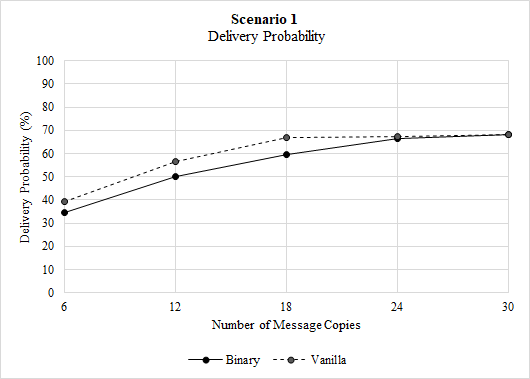
\includegraphics[width=.98\linewidth]{Results/Graphs/DeliveryProbability/S1_DeliveryProbability_SprayAndWaitComparison.png}
  \captionof{figure}{Comparison of delivery probability between vanilla and binary spray-and-wait in scenario 1}
  \label{fig:test1}
\end{minipage}%
\begin{minipage}[t]{.5\textwidth}
  \centering
  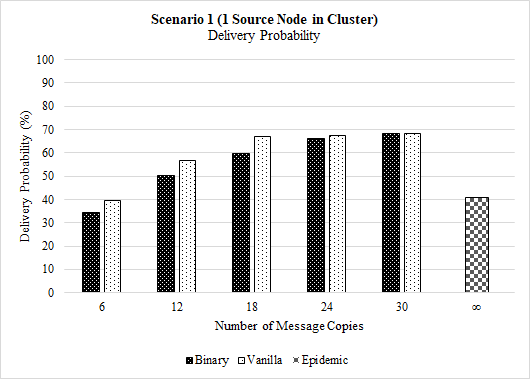
\includegraphics[width=.98\linewidth]{Results/Graphs/DeliveryProbability/S1_DeliveryProbability_AllComparison.png}
  \captionof{figure}{Comparison of delivery probability across all protocols in scenario 1}
  \label{fig:test2}
\end{minipage}

\centering
\begin{minipage}[t]{.5\textwidth}
  \centering
  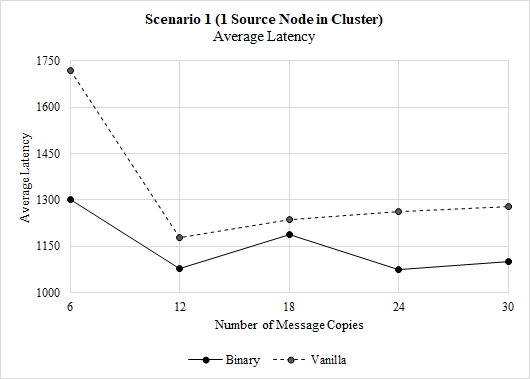
\includegraphics[width=.98\linewidth]{Results/Graphs/AverageLatency/S1_AverageLatency_SprayAndWaitComparison.png}
  \captionof{figure}{Comparison of average latency between vanilla and binary spray-and-wait over various message copies in scenario 1}
  \label{fig:test1}
\end{minipage}%
\begin{minipage}[t]{.5\textwidth}
  \centering
  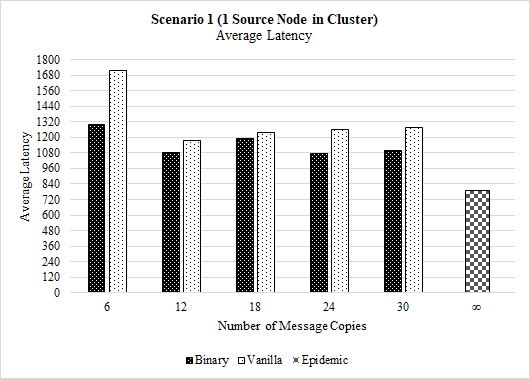
\includegraphics[width=.98\linewidth]{Results/Graphs/AverageLatency/S1_AverageLatency_AllComparison.png}
  \captionof{figure}{Comparison of average latency across all protocols in scenario 1}
  \label{fig:test2}
\end{minipage}

\centering
\begin{minipage}[t]{.5\textwidth}
  \centering
  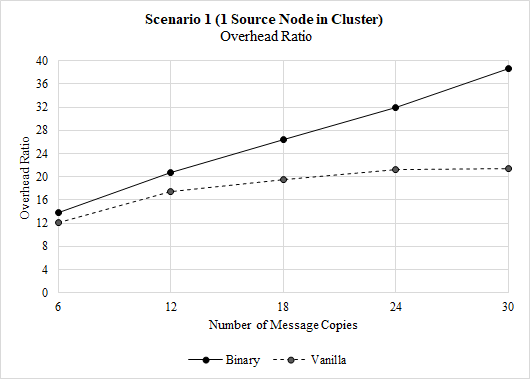
\includegraphics[width=.98\linewidth]{Results/Graphs/OverheadRatio/S1_OverheadRatio_SprayAndWaitComparison.png}
  \captionof{figure}{Comparison of overhead ratio between vanilla and binary spray-and-wait over various message copies in scenario 1}
  \label{fig:test1}
\end{minipage}%
\begin{minipage}[t]{.5\textwidth}
  \centering
  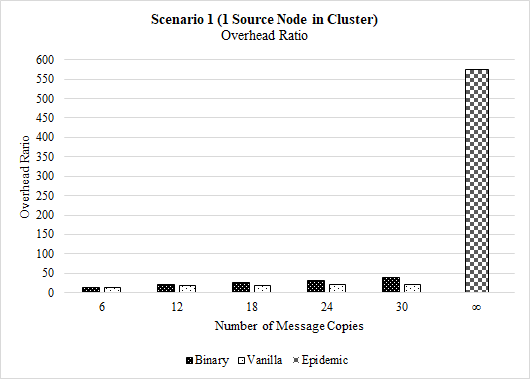
\includegraphics[width=.98\linewidth]{Results/Graphs/OverheadRatio/S1_OverheadRatio_AllComparison.png}
  \captionof{figure}{Comparison of overhead ratio across all protocols in scenario 1}
  \label{fig:test2}
\end{minipage}

\centering
\begin{minipage}[t]{.5\textwidth}
  \centering
  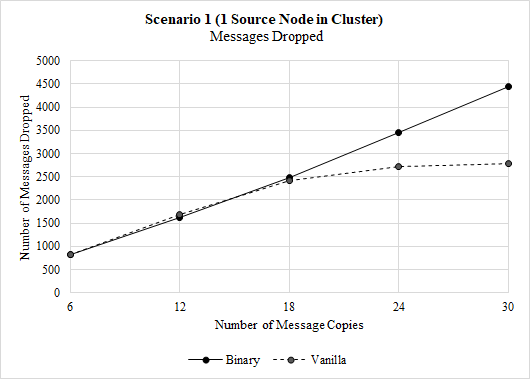
\includegraphics[width=.98\linewidth]{Results/Graphs/MessagesDropped/S1_MessagesDropped_SprayAndWaitComparison.png}
  \captionof{figure}{Comparison of messages dropped between vanilla and binary spray-and-wait over various message copies in scenario 1}
  \label{fig:test1}
\end{minipage}%
\begin{minipage}[t]{.5\textwidth}
  \centering
  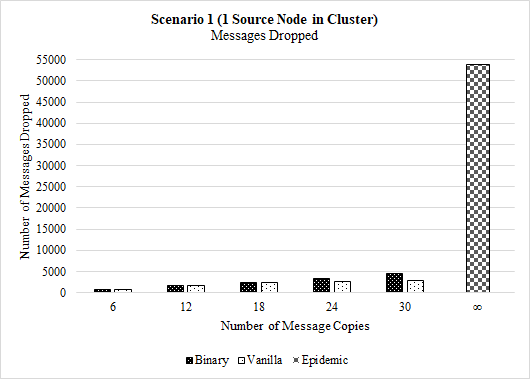
\includegraphics[width=.98\linewidth]{Results/Graphs/MessagesDropped/S1_MessagesDropped_AllComparison.png}
  \captionof{figure}{Comparison of messages dropped across all protocols in scenario 1}
  \label{fig:test2}
\end{minipage}

\end{figure}

\restoregeometry

\clearpage

\subsection{Scenario 2}
In this scenario, 10 trapped victims are simulated by a single node each. Each node moves randomly within a small pre-defined range and is able to create its own messages.

\begin{center}
\captionof{table}{Performance data for the epidemic routing protocol in scenario 2}
\vspace{6px}
\begin{tabular}{|r|c|}
\hline
\textbf{Parameter} & \textbf{Epidemic} \\ \hline
Messages Created & 243 \\ \hline
Messages Started & 329498 \\ \hline
Messages Relayed & 329491 \\ \hline
Messages Dropped & 326090 \\ \hline
Messages Delivered & 91 \\ \hline
Delivery Probability & 37.5\%\\ \hline
Overhead Ratio & 3619.8 \\ \hline
Average Latency & 1083.9 \\ \hline
Median Hop Count & 16 \\ \hline
\end{tabular}
\end{center}

\begin{center}
\captionof{table}{Performance data for the binary spray-and-wait routing protocol in scenario 2 using different values for the message copy limit}
\vspace{6px}
\begin{tabular}{|r|c|c|c|c|c|}
\hline
\textbf{Parameter} & \textbf{SWB6} & \textbf{SWB12} & \textbf{SWB18} & \textbf{SWB24} & \textbf{SWB30} \\ \hline
Messages Created & 243 & 243 & 243 & 243 & 243 \\ \hline
Messages Started & 1215 & 2714 & 4212 & 5648 & 6940 \\ \hline
Messages Relayed & 1215 & 2714 & 4212 & 5648 & 6940 \\ \hline
Messages Dropped & 1124 & 2332 & 3088 & 4026 & 5090 \\ \hline
Messages Delivered & 0 & 45 & 115 & 163 & 169 \\ \hline
Delivery Probability & 0\% & 18.5\% & 47.3\% & 67.1\% & 69.6\% \\ \hline
Overhead Ratio & N/A & 59.3 & 35.6 & 33.7 & 40.1 \\ \hline
Average Latency & N/A & 1621.4 & 1464.7 & 1392.1 & 1316.6 \\ \hline
Median Hop Count & 0 & 4 & 4 & 4 & 4 \\ \hline
\end{tabular}
\end{center}

\begin{center}
\captionof{table}{Performance data for the vanilla spray-and-wait routing protocol in scenario 2 using different values for the message copy limit}
\vspace{6px}
\begin{tabular}{|r|c|c|c|c|c|}
\hline
\textbf{Parameter} & \textbf{SWV6} & \textbf{SWV12} & \textbf{SWV18} & \textbf{SWV24} & \textbf{SWV30} \\ \hline
Messages Created & 243 & 243 & 243 & 243 & 243 \\ \hline
Messages Started & 1215 & 2703 & 4154 & 5418 & 6158 \\ \hline
Messages Relayed & 1215 & 2703 & 4154 & 5418 & 6158 \\ \hline
Messages Dropped & 1122 & 2324 & 3079 & 3976 & 4728 \\ \hline
Messages Delivered & 0 & 35 & 100 & 122 & 121 \\ \hline
Delivery Probability & 0\% & 14.4\% & 41.2\% & 50.2\% & 49.8\% \\ \hline
Overhead Ratio & N/A & 76.2 & 40.5 & 43.4 & 49.9 \\ \hline
Average Latency & N/A & 1592.8 & 1667.1 & 1536.2 & 1514.8 \\ \hline
Median Hop Count & 0 & 2 & 2 & 2 & 2 \\ \hline
\end{tabular}
\end{center}

\newpage

\noindent Scenario 2 increased the number of source nodes in the cluster from 1 to 10. The aim of this simulation was to compare the effectiveness of all 3 protocols when messages are created by a high-density cluster of source nodes rather than a single node. The simulation was designed to mimic real-life scenarios which involve large amounts of active mobile devices in close proximity to each other in an enclosed space.\\
\newline With the addition of the extra source nodes, epidemic's delivery probability fell from 40.7\%, seen in scenario 1, to 37.5\%, delivering only 91 messages (Figure 17). Additionally, epidemic's hop count increased from 6 to 16 (Table 4), the overhead ratio increased by 500\% (574.5 to 3619.8) (Figure 21) and the number of dropped messages exceeded 300,000 (Figure 23). It is clear from this data that high-density clusters of source nodes lead to exponential growth in the number of message transfers that the epidemic protocol attempts to create (Table 4), leading to completely unmanagable levels of overhead and considerably poorer performance. Epidemic is not a suitable routing protocol in scenarios which involve high-density source node clusters.\\
\newline All 5 simulations for both vanilla and binary spray-and-wait started with 6 message copies and increased the amount by 6 each time, finally reaching a total of 30 message copies. Interestingly, when using just 6 message copies both versions of spray-and-wait engaged in the exact same number of message transfers (1215) but achieved 0 message deliveries (Figure 16). On closer inspection it was discovered that no messages were able to leave the confines of the source node cluster. The cause was clear: the message copy limit had been reached simply by transferring created messages to the other source nodes contained in the cluster. For messages to reach nodes outside of the cluster, the number of spray-and-wait message copies should exceed the number of source nodes in the cluster. This was proven true by the next simulation which increased the number of message copies to 12:\\
\newline In scenario 1, both versions of spray-and-wait achieved a delivery probability of more than 50\% with 12 message copies (Figure 8). However, with a cluster of 10 source nodes, the protocols only managed 18.5\% (binary) and 14.4\% (vanilla) (Figure 16). However, increasing the number of message copies in later simulations saw the delivery probability for binary spray-and-wait reach comparable levels of the delivery probability seen in scenario 1, even exceeding them when using 24 and 30 message copies. The highest delivery probability achieved by binary was 69.6\% with 30 message copies (compared to 68.3\% with 30 message copies seen in scenario 1). Vanilla on the other hand reached a maximum delivery probability of only 50.2\% with 24 message copies (compared to 60.3\% with 30 message copies in scenario 1) and actually worsens with 30 message copies, producing only 49.8\% (Figure 16).\\
\newline In Scenario 1, the two spray-and-wait versions achieved similar performance, yet vanilla only slightly outperformed binary. However, in scenario 2, it is clear that binary performed considerably better than vanilla. It achieved a higher delivery probability (Figure 16), lower overhead ratio (Figure 20) and lower average latency (Figure 18). Performing at its best (30 message copies) binary achieved an overhead ratio of 40.1 which is only 4\% greater than its overhead ratio of 30.6 achieved in scenario 1 (Figure 12). Additionally, the average latency of 1316.6 is 19\% greater than the latency of 1102 achieved in scenario 1 (Figure 10). The median hop count doubled from 2 to 4 which may be the cause of the increased latency (Table 2 and Table 5).\\
\newline With a high-density cluster of 10 source nodes it is clear that binary spray-and-wait performs the best out of the 3 protocols, improving its delivery probability over single source nodes with only a small increase in overhead and latency. However, with a greater number of source nodes in the cluster, must come an increase in the message copy limit. Vanilla performed far poorer than it did with a single source node with a greatly decreased delivery probability. Epidemic's overhead increased exponentially and it achieved an extremely poor delivery probability.

\newgeometry{top=1cm}

\begin{figure}[h!]

\thispagestyle{empty}
\captionsetup{justification=centering, font=footnotesize}

\centering
\begin{minipage}[t]{.5\textwidth}
  \centering
  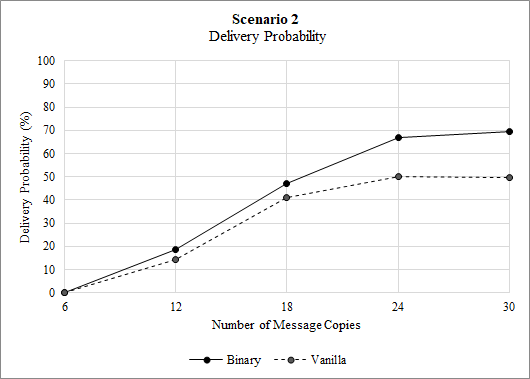
\includegraphics[width=.98\linewidth]{Results/Graphs/DeliveryProbability/S2_DeliveryProbability_SprayAndWaitComparison.png}
  \captionof{figure}{Comparison of delivery probability between vanilla and binary spray-and-wait in scenario 2}
  \label{fig:test1}
\end{minipage}%
\begin{minipage}[t]{.5\textwidth}
  \centering
  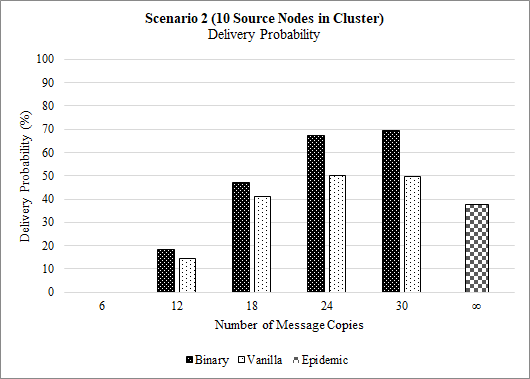
\includegraphics[width=.98\linewidth]{Results/Graphs/DeliveryProbability/S2_DeliveryProbability_AllComparison.png}
  \captionof{figure}{Comparison of delivery probability across all protocols in scenario 2}
  \label{fig:test2}
\end{minipage}

\centering
\begin{minipage}[t]{.5\textwidth}
  \centering
  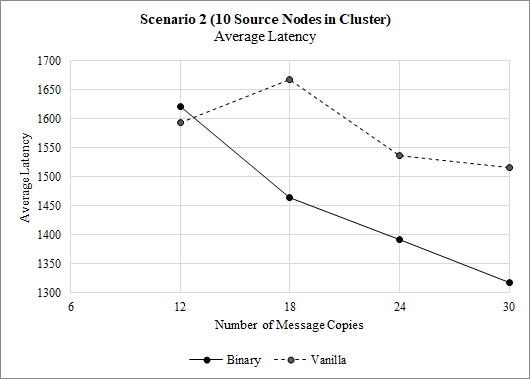
\includegraphics[width=.98\linewidth]{Results/Graphs/AverageLatency/S2_AverageLatency_SprayAndWaitComparison.png}
  \captionof{figure}{Comparison of average latency between vanilla and binary spray-and-wait over various message copies in scenario 2}
  \label{fig:test1}
\end{minipage}%
\begin{minipage}[t]{.5\textwidth}
  \centering
  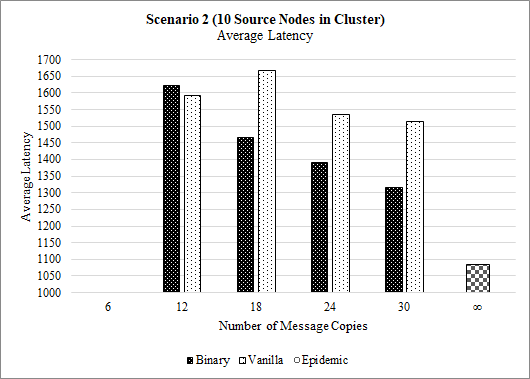
\includegraphics[width=.98\linewidth]{Results/Graphs/AverageLatency/S2_AverageLatency_AllComparison.png}
  \captionof{figure}{Comparison of average latency across all protocols in scenario 2}
  \label{fig:test2}
\end{minipage}

\centering
\begin{minipage}[t]{.5\textwidth}
  \centering
  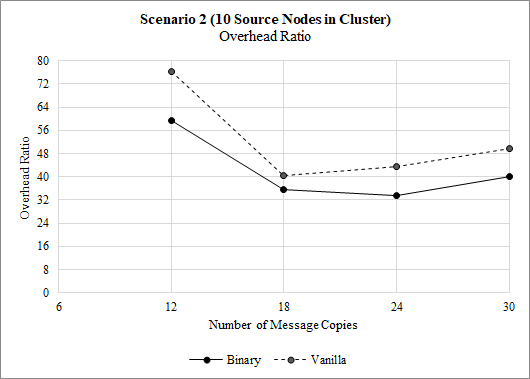
\includegraphics[width=.98\linewidth]{Results/Graphs/OverheadRatio/S2_OverheadRatio_SprayAndWaitComparison.png}
  \captionof{figure}{Comparison of overhead ratio between vanilla and binary spray-and-wait over various message copies in scenario 2}
  \label{fig:test1}
\end{minipage}%
\begin{minipage}[t]{.5\textwidth}
  \centering
  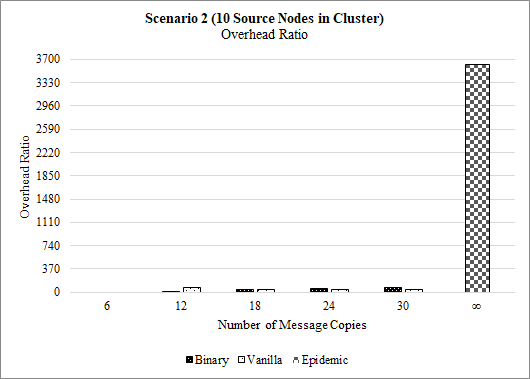
\includegraphics[width=.98\linewidth]{Results/Graphs/OverheadRatio/S2_OverheadRatio_AllComparison.png}
  \captionof{figure}{Comparison of overhead ratio across all protocols in scenario 2}
  \label{fig:test2}
\end{minipage}

\centering
\begin{minipage}[t]{.5\textwidth}
  \centering
  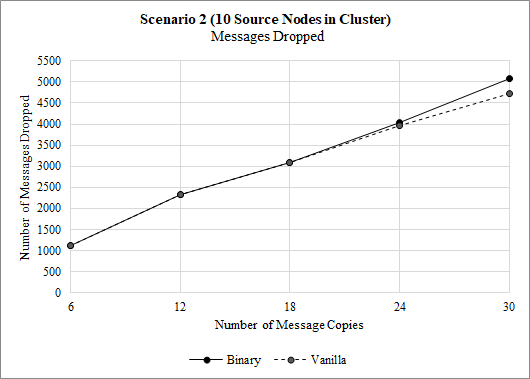
\includegraphics[width=.98\linewidth]{Results/Graphs/MessagesDropped/S2_MessagesDropped_SprayAndWaitComparison.png}
  \captionof{figure}{Comparison of messages dropped between vanilla and binary spray-and-wait over various message copies in scenario 2}
  \label{fig:test1}
\end{minipage}%
\begin{minipage}[t]{.5\textwidth}
  \centering
  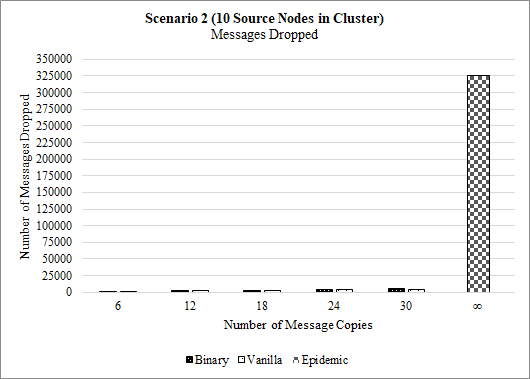
\includegraphics[width=.98\linewidth]{Results/Graphs/MessagesDropped/S2_MessagesDropped_AllComparison.png}
  \captionof{figure}{Comparison of messages dropped across all protocols in scenario 2}
  \label{fig:test2}
\end{minipage}

\end{figure}

\restoregeometry

\clearpage

\subsection{Scenario 3}
In this scenario, 20 trapped victims are simulated by a single node each. Each node moves randomly within a small pre-defined range and is able to create its own messages.

\begin{center}
\captionof{table}{Performance data for the epidemic routing protocol in scenario 3}
\vspace{6px}
\begin{tabular}{|r|c|}
\hline
\textbf{Parameter} & \textbf{Epidemic} \\ \hline
Messages Created & 243 \\ \hline
Messages Started & 600047 \\ \hline
Messages Relayed & 600034 \\ \hline
Messages Dropped & 596036 \\ \hline
Messages Delivered & 90 \\ \hline
Delivery Probability & 37\%\\ \hline
Overhead Ratio & 6666.0 \\ \hline
Average Latency & 1052.1 \\ \hline
Median Hop Count & 11 \\ \hline
\end{tabular}
\end{center}

\begin{center}
\captionof{table}{Performance data for the binary spray-and-wait routing protocol in scenario 3 using different values for the message copy limit}
\vspace{6px}
\begin{tabular}{|r|c|c|c|c|c|}
\hline
\textbf{Parameter} & \textbf{SWB12} & \textbf{SWB24} & \textbf{SWB36} & \textbf{SWB48} & \textbf{SWB60} \\ \hline
Messages Created & 243 & 243 & 243 & 243 & 243 \\ \hline
Messages Started & 2673 & 5632 & 8463 & 10847 & 12083 \\ \hline
Messages Relayed & 2673 & 5632 & 8463 & 10847 & 12082 \\ \hline
Messages Dropped & 2250 & 4668 & 6400 & 8368 & 9572 \\ \hline
Messages Delivered & 0 & 60 & 127 & 155 & 148 \\ \hline
Delivery Probability & 0\% & 24.7\% & 52.3\% & 63.8\% & 60.9\% \\ \hline
Overhead Ratio & N/A & 92.9 & 65.6 & 69.0 & 80.6 \\ \hline
Average Latency & N/A & 1589.3 & 1421.1 & 1400.4 & 1409.0 \\ \hline
Median Hop Count & 0 & 5 & 5 & 5 & 5 \\ \hline
\end{tabular}
\end{center}

\begin{center}
\captionof{table}{Performance data for the vanilla spray-and-wait routing protocol in scenario 3 using different values for the message copy limit}
\vspace{6px}
\begin{tabular}{|r|c|c|c|c|c|}
\hline
\textbf{Parameter} & \textbf{SWV12} & \textbf{SWV24} & \textbf{SWV36} & \textbf{SWV48} & \textbf{SWV60} \\ \hline
Messages Created & 243 & 243 & 243 & 243 & 243 \\ \hline
Messages Started & 2676 & 5623 & 8240 & 9588 & 9809 \\ \hline
Messages Relayed & 2676 & 5623 & 8240 & 9588 & 9809 \\ \hline
Messages Dropped & 2246 & 4656 & 6414 & 7746 & 7987 \\ \hline
Messages Delivered & 3 & 58 & 101 & 105 & 111 \\ \hline
Delivery Probability & 1.2\% & 23.9\% & 41.6\% & 43.2\% & 45.7\% \\ \hline
Overhead Ratio & 891.0 & 95.9 & 80.6 & 90.3 & 87.4 \\ \hline
Average Latency & 1834.4 & 1660.8 & 1482.6 & 1491.6 & 1544.6 \\ \hline
Median Hop Count & 2 & 2 & 2 & 2 & 2 \\ \hline
\end{tabular}
\end{center}

\newpage

\noindent Scenario 3 increased the number of source nodes in the cluster from 10 to 20. The aim of this simulation was to compare the effectiveness of all 3 protocols when messages are created by an even higher density cluster of source nodes. Note that, to keep the simulations accurate, the number of message copies for this scenario started at 12 and increased by 12 each time, finally reaching 60 message copies. This ensured that the difference between the number of message copies and the number of source nodes in the cluster was proportional to the difference seen in the previous simulation.\\
\newline Similar to scenario 2, epidemic performs extremely poorly; its delivery probability falling another 0.5\% from 37.5\% to 37\% (Figure 25). This time, the overhead ratio increased by 84\% from (3619.8 in scenario 2 to 6666) (Figure 29) and the number of dropped messages nearly doubled (Figure 31). Interestingly, the median hop count (Table 7) and average latency (Figure 27) actually decreased. However, the facts remain the same: with such a low delivery probability, epidemic is unsuitable for situations involving high-density source node clusters.\\
\newline All 5 simulations for both vanilla and binary spray-and-wait started with 12 message copies and increased the amount by 12 each time, reaching a total of 60 message copies. In scenario 2, it was observed that a quantity of message copies fewer than the number of source nodes in the cluster resulted in 0 deliveries for spray-and-wait versions (Figure 16). In this scenario, with 20 source nodes and 16 message copies, binary performs similarly; delivering 0 messages. However, surprisingly, vanilla managed to deliver 3 messages (achieving a delivery probability of 1.2\%) (Figure 25). This is almost certainly a result of the different propogation methods used by each version. In this specific scenario, vanilla spray-and-wait managed to transfer multiple messages to nodes outside of the source cluster before reaching the message copy limit, whereas binary failed to do so. Despite this, a delivery probability of 1.2\% is so negligable that it hardly warrants the consideration of vanilla spray-and-wait (with 12 message copies) as a valid protocol for this scenario; the message count needs to be raised.\\
\newline Binary spray-and-wait achieves its maximum delivery probability of 63.8\% with a message count of 48, but decreases to 60.9\% when using a count of 60. However, vanilla reaches its maximum delivery probability of 45.7\% with a message count of 60 (Figure 24). Both protocols' maximum delivery probability is slightly less than their scenario 2 maximums (Figure 16) (binary dropped from 69.6\% to 63.8\%, a decrease of 8\%, and vanilla dropped from 50.2\% to 45.7\%, a decrease of 9\%). It's possible that a greater delivery probability may be achieved by using intermediate values, between the ones used in this experiment. Nevertheless, the data gathered in this experiment suggests that if the number of source nodes in the cluster increases, the number of message copies used by either protocol should also be increased to compensate.\\
\newline Due to the increased number of message copies and the 10 extra source nodes, the number of messages dropped by both protocols also increased significantly when compared to the results of scenario 2 (Figure 22 and Figure 30). At 60 message copies, vanilla spray-and-wait dropped 7987 messages compared to 4728 in scenario 2 (an increase of 59\%) and binary dropped 9572 compared to 5090 (an increase of 53\%). The increase in messages relays and drops also had an affect on the overhead ratio. At 60 message copies, vanilla spray-and-wait had an overhead ratio of 87.4 (an increase of 57\%) and binary had an overhead ratio of 80.6 (an increase of 50\%) (Figure 28). Comparing both versions of spray-and-wait for scenario 2 and scenario 3, both the overhead ratio and number of messages dropped increased by a range of 50\%-59\%. This suggests that, regardless of the version used, increasing the number of message copies to compensate for the increased number of source nodes leads the protocol to scale in a predictable way. Further tests that simulate even denser source clusters with a higher number of message copies should be conducted to explore this hypothesis.\\
\newline Finally, similar conclusions to scenario 2 can be found here: binary spray-and-wait outperforms both vanilla and epidemic. It achieves a considerably higher delivery probability as well as lower overhead and average latency.

\newgeometry{top=1cm}

\begin{figure}[h!]
\thispagestyle{empty}
\captionsetup{justification=centering, font=footnotesize}

\centering
\begin{minipage}[t]{.5\textwidth}
  \centering
  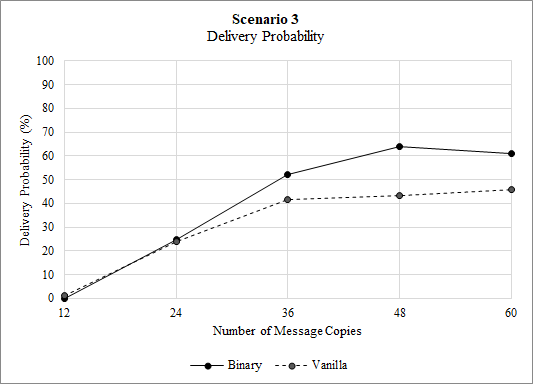
\includegraphics[width=.98\linewidth]{Results/Graphs/DeliveryProbability/S3_DeliveryProbability_SprayAndWaitComparison.png}
  \captionof{figure}{Comparison of delivery probability between vanilla and binary spray-and-wait in scenario 3}
  \label{fig:test1}
\end{minipage}%
\begin{minipage}[t]{.5\textwidth}
  \centering
  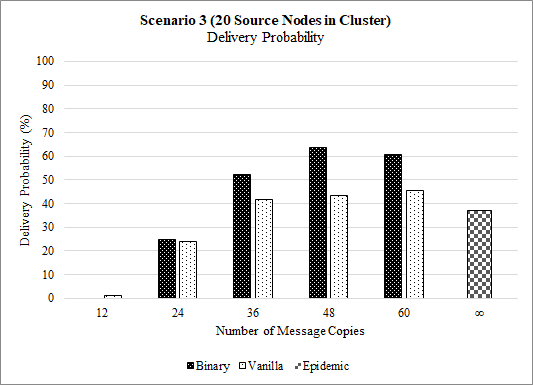
\includegraphics[width=.98\linewidth]{Results/Graphs/DeliveryProbability/S3_DeliveryProbability_AllComparison.png}
  \captionof{figure}{Comparison of delivery probability across all protocols in scenario 3}
  \label{fig:test2}
\end{minipage}

\centering
\begin{minipage}[t]{.5\textwidth}
  \centering
  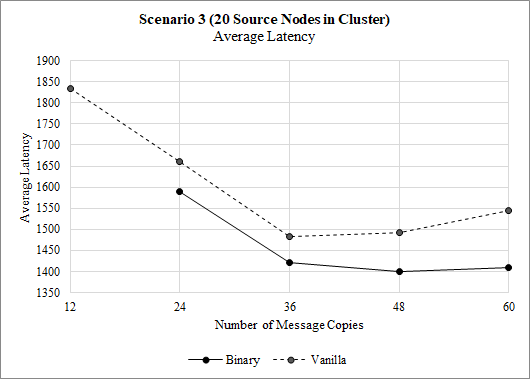
\includegraphics[width=.98\linewidth]{Results/Graphs/AverageLatency/S3_AverageLatency_SprayAndWaitComparison.png}
  \captionof{figure}{Comparison of average latency between vanilla and binary spray-and-wait over various message copies in scenario 3}
  \label{fig:test1}
\end{minipage}%
\begin{minipage}[t]{.5\textwidth}
  \centering
  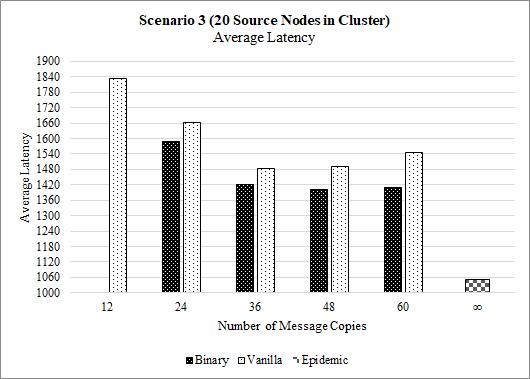
\includegraphics[width=.98\linewidth]{Results/Graphs/AverageLatency/S3_AverageLatency_AllComparison.png}
  \captionof{figure}{Comparison of average latency across all protocols in scenario 3}
  \label{fig:test2}
\end{minipage}

\centering
\begin{minipage}[t]{.5\textwidth}
  \centering
  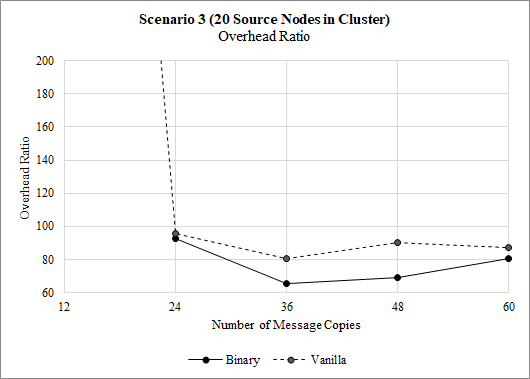
\includegraphics[width=.98\linewidth]{Results/Graphs/OverheadRatio/S3_OverheadRatio_SprayAndWaitComparison.png}
  \captionof{figure}{Comparison of overhead ratio between vanilla and binary spray-and-wait over various message copies in scenario 3}
  \label{fig:test1}
\end{minipage}%
\begin{minipage}[t]{.5\textwidth}
  \centering
  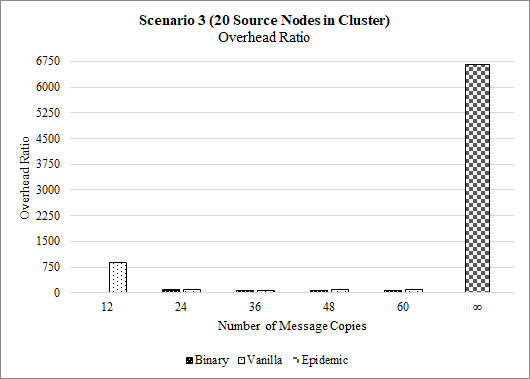
\includegraphics[width=.98\linewidth]{Results/Graphs/OverheadRatio/S3_OverheadRatio_AllComparison.png}
  \captionof{figure}{Comparison of overhead ratio across all protocols in scenario 3}
  \label{fig:test2}
\end{minipage}

\centering
\begin{minipage}[t]{.5\textwidth}
  \centering
  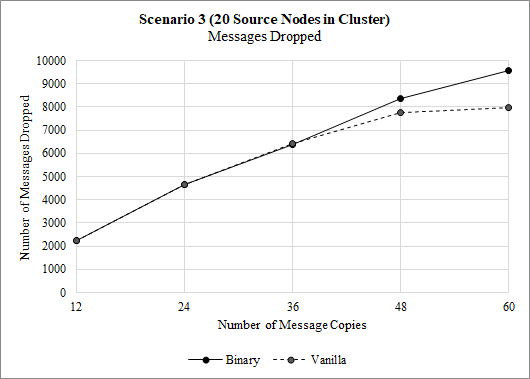
\includegraphics[width=.98\linewidth]{Results/Graphs/MessagesDropped/S3_MessagesDropped_SprayAndWaitComparison.png}
  \captionof{figure}{Comparison of messages dropped between vanilla and binary spray-and-wait over various message copies in scenario 3}
  \label{fig:test1}
\end{minipage}%
\begin{minipage}[t]{.5\textwidth}
  \centering
  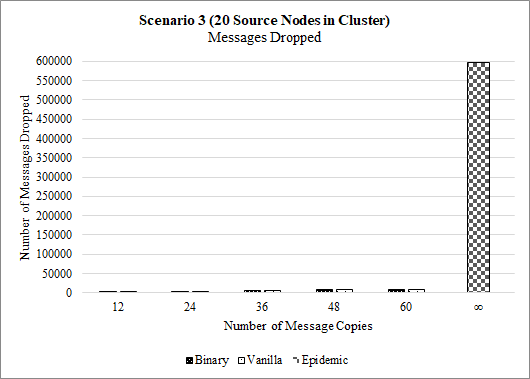
\includegraphics[width=.98\linewidth]{Results/Graphs/MessagesDropped/S3_MessagesDropped_AllComparison.png}
  \captionof{figure}{Comparison of messages dropped across all protocols in scenario 3}
  \label{fig:test2}
\end{minipage}

\end{figure}

\restoregeometry

\clearpage

\section{Conclusion - Pros and Cons}
This experiment simulated a critical situation involving an increasingly high-density cluster of trapped civilians who required immediate rescue and assistance from emergency services. The scenario was modelled in the ONE simulator and 3 different routing protocols (epidemic, vanilla spray-and-wait and binary spray-and-wait) were used to relay messages from the victims to a destination node at the local hospital. The scenario consisted of 3 variations: 1 source node, 10 source nodes, and 20 source nodes. The aim of the experiment was to evaluate the performance characteristics of each routing protocol when there are an increasing number of sources nodes located in close proximity to each other.\\
\newline Epidemic performed noticeably poorer than both vanilla and binary spray-and-wait in all 3 scenarios, never achieving a delivery probability of more than 40.7\%. As a result of its uncontrolled replicative behaviour, it engaged in an exponentially increasing number of message transfers as the number of source nodes was increased, numbering over 500,000 in the third scenario. Due to the sheer quantity of message copies, the network became heavily congested and most nodes reached their maximum buffer occupancy. This also produced unmanageable overhead and increased the median hop count for message travel. Despite all these cons, epidemic did produce a lower average latency then every spray-and-wait test conducted across all 3 scenarios. Regardless, it is very clear that epidemic is not an appropriate routing protocol for use in emergency situations involving high-density source node clusters.\\
\newline With just one source node in the cluster, vanilla spray-and-wait only marginally outperformed its binary counterpart, achieving the same delivery probability of 68.3\% (with 30 message copies) but doing so with less overhead, message drops, and a lower median hop count. However, as soon as multiple source nodes were introduced to the cluster, binary spray-and-wait quickly outperformed vanilla, achieving 15-20\% higher delivery probabilities when using the maximum number of message copies tested (30 in scenario 2 and 60 in scenario 3). Despite dropping more messages, binary also achieved a lower overhead ratio and average latency than vanilla.\\
\newline The data collected from this experiment strongly suggests that, out of the 3 protocols tested, binary spray-and-wait is the best protocol for use in emergency situations involving high-density source node clusters, primarily due its good delivery probability. Binary does have some disadvantages however: particularly the fact that, on average, it drops more messages than vanilla spray-and-wait and has a higher median hop count. The data also suggests that to maintain a higher delivery probability it is necessary to increase the number of message copies disseminated by the spray-and-wait protocol in proportion to the number of source nodes in the cluster. Additional tests involving higher density source clusters should be conducted in order to further explore this hypothesis and ascertain whether the binary spray-and-wait protocol scales manageably when the network size and number of nodes increases.

\section{Wider Discussion - The Benefits of Opportunistic Networks for Mass Animal Monitoring}
Opportunistic networks, particularly DTNs, are focused on bringing reliable networking to non-traditional, usually extreme environments which typically struggle with significant delay and disruption and where standard procotols such as TCP [3] are unsuitable. Over the past several decades, especially with the increased pervasiveness of the internet, opportunistic network technologies and protocols have seen more and more development and success, being deployed around the world in new and exciting scenarios. In this section, a wider discussion explores the application of opportunistic networks for mass animal monitoring; the tracking and recording of large groups of animals over huge distances.\\

\subsection{Automated Cattle Monitoring}

\noindent In the UK, the monitoring of cattle is needed for the detection of health problems such as infections, diseases and lameness which could potentially lead to decreased productivity or livestock death. Currently, farm-level monitoring systems are non-obligatory, heterogeneous, and often poorly integrated. Some advanced enterprises utilise milk monitoring with stationary or animal mounted sensors, but these have very short to medium ranges and experience frequent disconnections [20].\\

\noindent Researchers at the University of Nottingham have proposed a delay store-and-forward architecture for solving many of the issues related to the mass monitoring of cattle based around an energy efficient, disruption tolerant MANET routing protocol that allows for the minimising and balancing of energy utilisation [20]. This protocol works by ``offloading data for long-term storage by sending data to farm servers via sinks that are a part of the MANET''. The researchers also found that, by minimising energy consumption in the face of low data traffic and high node mobility, the labour intensity of the architecture's maintenance could be reduced, allowing the batteries installed in the animal-mounted devices to be changed less frequently. This was achieved by dynamically adapting the protocol to the behaviour of the animals being monitored by ``utilising the heterogeneity of nodes' mobility, selecting routes with the longest lifetime and opportunistic route discovery''.\\

\noindent The proposed architecture itself is decentralised and consists of multiple MANETs containing mobile sensor nodes, usually mounted on animals. These sensors acquire, store and process data related to the animal's health and location and are able to cache both measured and queried data. Queries usually concern specific animals, or a collection of animals over a specific area and can be issued by remote users over the internet via a peer-to-peer internet overlay that connects each farm MANET. Typical users of the system would include farmers, slaughter workers and anyone involved in the animal trade.

\subsection{ZebraNet}

ZebraNet is an active mobile, wireless sensor network aimed at improving tracking 
technology for wildlife tracking [4][21]. As its name suggests, ZebraNet's primary focus is the monitoring of zebra across huge regions of Africa whilst managing the difficult deployment, lack of communication infrastructure, and coordination of many static and mobile sensors. The ZebraNet system includes custom tracking collars (the mobile nodes in the network) which are mounted on the Zebra in the study. The collars communicate in a peer-to-peer fashion to deliver logged data back to researchers at a mobile ``base station''. Each collar has GPS, memory (containing a lighweight operating system), a wireless network interface, and a CPU. These components allow each node to act as a minimalistic computing device in its own right [21].\\

\noindent Most importantly, ZebraNet displays many attributes of opportunistic networks, relying on periodic node discovery and peer-to-peer communication to relay data to the base station, utilising store-and-forward routing rather than constant communication access. Instead of connection-oriented protocols, such as TCP, which identify end-to-end routes between source and destination, ZebraNet transmits data in a single-hop fashion via other nodes and opportunistic heuristics involving historical data of the mobile base station's last known location. The network environment can be seen as extreme due to its very large scale and relative sparsity (groups of Zebra may be located many hundreds of kilometres away from each other). Some results of this non-traditional environment are frequent risks of disconnections and large latency between communications. As a result, ZebraNet has some typical attributes of DTNs [21].\\

\noindent One of the goals of the ZebraNet project is to be energy-efficient, and use as few resources as possible whilst still maintaining a reliable system with high message delivery probability. To this end, ZebraNet's middleware layer (dubbed ``Impala'') was designed to encourage application ``modularity, simplicity, adaptivity, and repairability'' [21]. Impala allows for the scheduling of regular operations, handles unexpected and asynchronous events and unifies media access control and transport control into ``an efficient network protocol that supports a range of message models ... tailored to ZebraNet's application needs.'' [21]\\

\noindent To conclude, both the proposed cattle monitoring architecture and the ZebraNet project are examples of bespoke solutions to problems arising from the use of networking technologies in non-traditional, extreme environments. Both examples use aspects of opportunistic networks such as single-hop, opportunistic routing protocols in a peer-to-peer fashion, and focus on creating reliable systems which are energy-efficient and use minimal resources. 

\vspace{50px}

\addcontentsline{toc}{section}{References}
\begin{thebibliography}{20}

\bibitem{A Survey of Opportunistic Networks} 
Huang, C., Lan, K., \& Tsai, C. (2008).
``A Survey of Opportunistic Networks''
\textit{22nd International Conference on Advanced Information Networking and Applications - Workshops (aina workshops 2008)}, pp.1672-1677.

\bibitem{Delay- and Disruption-Tolerant Networking}
Farrell, S., \& Cahill, V. (2006).
``Delay- and Disruption-Tolerant Networking''
\textit{Artech House, Inc., Norwood, MA.}

\bibitem{TCP Protocol}
Postel, J. (1981).
``Transmission Control Protocol'', RFC 793.

\bibitem{ZebraNet}
Juang, P., Oki, H., Wang, Y., Martonosi, M., Shiuan Peh, L., \& Rubenstein, D. (2002).
``Energy-Efficient Computing for Wildlife Tracking: Design Tradeoffs and Early Experiences with ZebraNet'''
\textit{ACM SIGOPS Operating Systems Review} \textbf{36}(5), pp.96–107

\bibitem{Interplanetary Internet}
Jackson, J. (2005). 
``The Interplanetary Internet''
\textit{IEEE Spectrum}. Available at: https://spectrum.ieee.org/telecom/internet/the-interplanetary-internet [Accessed 24 Oct. 2018].

\bibitem{Mobile Ad-Hoc Networks}
Giordano, S (2002).
``Mobile Ad-Hoc Networks''
\textit{Handbook of Wireless Networks and Mobile Computing} pp.325-346

\bibitem{Trends in MANETs}
Singh, S., Dutta, S.C., \& Singh D.K. (2012). 
``A Study on Recent Research Trends in MANET''
\textit{International Journal of Research and Reviews in Computer Science (IJRRCS) \textbf{3}(3), pp.1654-1658} 

\bibitem{Security in MANETs}
Djenouri, D., Khelladi, L., \& Badache, A.N. (2005).
``A Survey of Security Issues in Mobile Ad Hoc and Sensor Networks''
\textit{IEEE Communications Surveys and Tutorials} \textbf{7}(4), pp.2-28

\bibitem{VANETs}
Dahiya, A., \& Chauhan, R.K. (2010).
``A Comparative Study of MANET and VANET Environment''
\textit{Journal of Computing} \textbf{2}(7), pp.87-92

\bibitem{Flooding vs Forwarding in DTNs}
Rani, S., \& Abhilasha (2015).
``Performance Evaluation of various Flooding and
Forwarding Protocols based on Delay Tolerant
Networks: A Review''
\textit{International Journal of Science and Research (IJSR)} \textbf{4}(7), pp.1625-1629

\bibitem{Epidemic}
Vahdat, A., \& Becker, D. (2000).
``Epidemic Routing for Partially-Connected Ad Hoc Networks''
\textit{Department of Computer Science, Duke University, Durham}

\bibitem{Epidemic Performance}
Zhang, X., Neglia, G., Kurose, J., \& Towsley, D. (2007).
``Performance Modelling of Epidemic Routing''
\textit{Computer Networks} \textbf{51}(10), pp.2867-2891

\bibitem{Spray and Wait}
Spyropoulos, T., Psounis, K., \& Raghavendra, C.S. (2005).
``Spray and Wait: An Efficient Routing Scheme for
Intermittently Connected Mobile Networks''
\textit{Proceedings of the 2005 ACM SIGCOMM Workshop on Delay-Tolerant Networking}, pp.252-259

\bibitem{ONE Sim}
Karänen, A. (2008).
``Opportunistic Network Environment Simulator''
\textit{Helsinki University of Technology, Department of Communications and Networking}

\bibitem{ONE Sim Website}
The ONE (Opportunistic Network Environment Simulator). Available at: https://akeranen.github.io/the-one/ [Accessed 4th Dec. 2018]

\bibitem{802.11b}
Jiang, D. \& Delgrossi, L. (2008).
``IEEE 802.11p: Towards an International Standard for Wireless Access in Vehicular Environments.'' 
\textit{In: Vehicular Technology Conference, 2008. VTC Spring 2008. IEEE}, pp 2036-2040.

\bibitem{WAVE}
CA Engineering - 802.11p Automotive. Available at: https://www.caengineering.com/technologies/?a=802.11-wi-fi\&id=802.11p-automotive [Accessed 9th Dec. 2018]

\bibitem{OPPNETS}
Pelusi, L., Passarella, A., \& Conti, M. (2006).
``Opportunistic Networking: Data Forwarding in Disconnected Mobile Ad Hoc Networks''
\textit{IEEE Communications Magazine archive \textbf{44}(1), November 2006}, pp.134-141.

\bibitem{StoreAndForward}
Warthman, F. (2012).
``Delay-and Disruption-Tolerant Networks (DTNs) - A Tutorial'' \textit{Interplanetary Internet Special Interest Group, 2012}

\bibitem{Cattle}
Wietrzyk, B. \& Radenkovic, M. (2010)
``Realistic Large Scale ad hoc Animal Monitoring''
\textit{In: International Journal on Advances in Life Sciences, \textbf{2}(1 \& 2)}

\bibitem{ZebraNet Website}
ZebraNet Introduction and Deployment Experience. Available at: https://www.ietf.org/mail-archive/web/dtn-interest/current/msg03702.html [Accessed 9th Dec. 2018]

\end{thebibliography}
 
\end{document}